% Overview figure (Fig. 1). Rendered by experiments/paper/make_overview.py
% (candidate A2) into figures/overview_A2.pdf, 7.16 in wide, fonts 7 pt body,
% 6.5 pt sub-text, 8 pt card titles, so it is placed at natural size and
% never scaled. Copy figures/overview_A2.pdf to Overleaf next to main.tex.
\begin{figure*}[t]
  \centering
  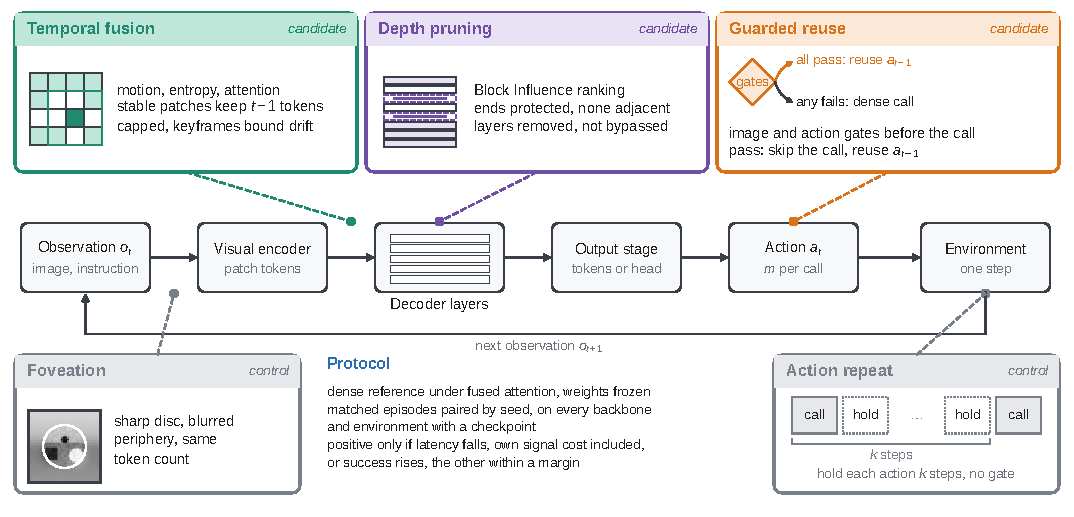
\includegraphics[width=\textwidth]{figures/overview_A2.pdf}
  \caption{Where each intervention enters a frozen VLA control loop.
  Candidates (top) act on the vision tokens, the decoder depth, and the
  policy call. Controls (bottom) act on the input image and on the action
  hold. Every variant is scored against the dense reference on matched
  episodes.}
  \label{fig:overview}
\end{figure*}
